\documentclass{beamer}
%\usetheme{Antibes}
\usetheme{Dresden}
%\usetheme{Frankfurt}
%\usetheme{Copenhagen}
%\usetheme{Darmstadt}
%\usecolortheme{dolphin}
\usepackage{cancel}
\usepackage{tikz}
%%%%%%%%%%%%%%%%%%%%%%%%%%%%%%%%%%%%%%%%%%%%%%%%%%%%%%%%
\usepackage{multicol}

\newtheorem{proposition}[theorem]{Proposition}
\newtheorem{remark}[theorem]{Remark}
\newtheorem*{remark*}{Remark}
\newtheorem{conjecture}[theorem]{Conjecture}
\newtheorem{claim}[theorem]{Claim}
\newtheorem*{claim*}{Claim}
\usepackage{xcolor}
\usepackage{longtable}
\usepackage{hyperref}
\newtheorem{openproblem}[theorem]{Open Problem}


\setbeamertemplate{blocks}[rounded][shadow=true]

\setbeamertemplate{theorems}[ams style]
\begin{document}
	\title[]{\textcolor{black}{\textbf{Classification of political articles.}}}
	
	\author[Yevgeniy Kostrov \hspace{1in} ekostrov@yahoo.com]
	{\textcolor{black}
		{\textbf{by Y.~Kostrov\inst}}}
	\date[April 14, 2019]
	
	%
	%	Title Page:
	%	
	
	%	{
		%\usebackgroundtemplate{\includegraphics[height=\paperheight,width=\paperwidth]{london}}
		%\frame{
			%}
		%}
	\begin{frame}	
		\maketitle
	\end{frame}
	\begin{frame}{\contentsname}
		\begin{multicols}{2}
			\tableofcontents
		\end{multicols}
	\end{frame}
	%
	%
	%	
	%
	%
	%}
\section{Overview}
\frame{
	\frametitle{Overview }
	%\begin{center}
		In this project,\\ I create a model that will classify political articles collected by me from different websites.\\
			\centering{ 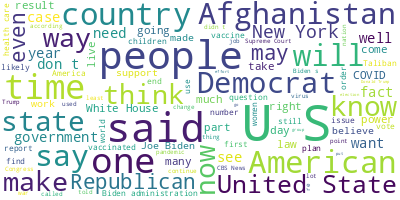
\includegraphics[width=2in]{cloud.png}}
	%\end{center}
}
\section{Business Problem}
\frame{
	\frametitle{Business Problem}
	\begin{itemize}
		\item This project is centered around understanding the political view of the short article that we can find on the internet. 
		\item It is, often, very hard to decide which political inclination the article has. 
		\item The reader can take the text and use the model that comes out of this project to confirm the understanding of the political notion that the user has after reading with the prediction of our model.
	\end{itemize}
}
\section{Data}
\frame{
	\frametitle{Data Used in the Project}
	\begin{itemize}
		\item The data for this project was collected by me from the following websites:
		\begin{itemize}
			\item 		 www.freebeacon.com, 
			\item www.americanthinker.com, 
			\item www.huffpost.com, 
			\item www.slate.com, 
			\item news.gallup.com, and
			\item  www.cbsnews.com.
		\end{itemize}
	\end{itemize}
}
\frame{
	\begin{itemize}
		\item I put the articles into three category based on the political view of the hosting website. 
		\item The categories are 
		\begin{itemize}
			\item "left", 
			\item "center"
			\item "right".
		\end{itemize}. 
	\item The data file has only two columns:
	\begin{itemize}
		\item "article"
		\item  "label"
	\end{itemize} 
	\end{itemize}
}
\frame{
	\frametitle{Distribution of Labels by Class}
	\begin{center}
		
\includegraphics[width=4in]{classDistBar.png}
	\end{center}
}
\frame{
	\frametitle{Pie Chart of Labels by Class}
	\begin{center}
		
\includegraphics[width=4.5in]{classDistPieChart.png}
	\end{center}
}
\frame{
	\frametitle{Sentiment analysis}
	Sentiment analysis (also known as opinion mining or emotion AI) is the use of natural language processing, text analysis, computational linguistics, and biometrics to systematically identify, extract, quantify, and study affective states and subjective information. (Wikipedia)
}
\frame{
	\frametitle{Overall Distribution of Sentiments}
	\begin{center}
		
\includegraphics[width=4in]{sentDistHist.png}
	\end{center}
}
\frame{
	\frametitle{Distribution of Average Sentiments by Class}
	\begin{center}
		
\includegraphics[width=3.5in]{sentByClassAver.png}
	\end{center}
}
\section{Modeling}
\frame{
	\frametitle{Modeling: Creating  Models}
	\begin{itemize}
		\item 	I have used four models: Naive Bayes, Support Vector Machines, Random Forest, and Convolutional Neural Network with Long Short Term Memory Layers  with different few different ways to modify text into numerical data suited for machine learning.  
		\item  I used accuracy as a primary metric for assessment of models.
	\end{itemize}
}

\frame{
	\frametitle{Explanation of  Accuracy}
	\begin{itemize}
		\item There is another metric we will use is called "accuracy".
		\item Accuracy is defined as:
		\[\small \text{Accuracy} = \frac{\text{Correct Predictions}}{\text{All Predictions}}\]
		\normalsize 
	\end{itemize}
}
\frame{
	\frametitle{Explanation of Accuracy}
	\begin{itemize}
		\item Accuracy is the number of correctly predicted data points out of all the data points.
	\end{itemize}
}

\section{Models' Performance}
\frame{
	\frametitle{How Well Models Performed}
	\begin{itemize}
			\item The best performance was achieved with the Support Vector Machines classifier at 98.7\% of accuracy.
	\end{itemize}
}
\section{Conclusions}
\frame{
	\frametitle{Business Suggestion}
	\begin{center}
		Based on my analysis, 
		\begin{itemize}
			\item I suggest to use Support Vector Machines model for the prediction of the political inclination of the article.
			\item The model can help internet users who are not sure about the flavor of the political news to verify what kind of an article they are reading.
		\end{itemize}
	\end{center}
	
}
\frame{
	\begin{center}
		\LARGE
		THE END \\
		THANK YOU!
	\end{center}
}
\end{document}